\part{The back end}\label{part:nstar}


\chapter{Introduction}\label{chap:nstar-abstract}

Assembly languages are the lowest level of humanly-possible programming there exists nowadays. They were used back in the days for very performance-critical tasks, or even just for fun, as there weren't many other programming languages available. Nowadays, with all the existing ones, most people have never used any assembly language.

Despite their apparent simplicity, and the small amount of work you need to put into creating assembly languages, those are in fact very hard to use. At that low level, there is no such thing as Java's exceptions keeping you from doing dumb things, Rust's linear types keeping you from leaking memory nor even Garbage Collectors. The nice things preventing you from having segfaults simply do not exist, and you are expected to either provide all those things yourself (creating a language runtime) or be very careful about what you are doing each time you write a single instruction (even a simple \texttt{mov} can have undesirable side-effects).

Doing dumb things is something that we must prevent directly when using the language. That way, we do not need to rely on external verification tools or debuggers, trying to know why a program segfaults at a specific point.
This is where a type system can become handy. Typed assembly languages are assembly languages augmented with simple yet powerful type system. Among the most famous typed assembly languages are TALx86~\cite{TALx86} and DTAL~\cite{DTAL}.

TALx86 is basically NASM with a type system, targetting only the x86 architecture. DTAL is much more complicated and embeds a completely dependent type system.

\vspace{\baselineskip}

N*'s goal is to assist users with a simple but powerful type system, as well as other features like what is called ``branch-checking'' which prevents from leaking the control flow of the program, and thus makes a part of the type-checking process meaningful.
But before even being a usable programming language, N* aims at being a compiler backend (much like for example LLVM), and is used that way in the Zilch project. Differences with other compiler backends are mostly the type-system, allowing the compilation of Zilch source code into type-safe instructions.

\vspace{\baselineskip}

Because N* supports compiling to multiple architectures, using different grammars, describing N* will at first be platform-agnostic, treating common aspects between all CPU architectures, and then will be divided into multiple categories, explaining in more details some features on a per-architecture basis\footnote{Note that the target executable format (ELF, PE, \ldots) is also considered as an architecture-specific thing, but should not influence N* much.}.

\chapter{Non platform-specific features}\label{chap:nstar-common}

\section{Introduction}\label{sec:nstar-common-introduction}

Before describing every platform-independent feature, we need to define some notation regarding inference rules:
\begin{itemize}
  \item $\Vdash$ is used to denote the kind inference process;
  \item $\Gamma$ is the kind typing context;
  \item $\vdash_{data}$ denotes the type inference process in the \texttt{data} (and \texttt{rodata}) sections;
\end{itemize}

\section{Types}\label{sec:nstar-common-ts}

One of the differences between classical assembly languages and N* is its type system.
Compared to other higher level programming languages like Java, C++, etc, N* has a very simple yet powerful and expressive enough type system.

In programming, types are used mostly to prove at compile-time that a given program should behave well if it type-checks. While this works for more elaborated programming languages like Haskell, Idris, etc, most type systems aren't expressive enough to absolutely guarantee that everything will work at run-time (in fact, there is no possible way of doing this, because for example a memory allocation may fail, and this cannot be checked at compile-time). However, we can try to guarantee as much as possible.

N* doesn't try to solve this issue, because it would be really hard to target a dependently typed assembly language from a non-dependently typed programming language. But where all used assembly languages do not even consider types (only numbers, in fact), N* embeds a powerful type system used to remove the possibility of bugs (like incorrect structure addresses passed as a parameter function, or incoherent types in some instructions).

\subsection{Kinds}\label{subsec:nstar-common-ts-kinds}

Kinds (also known as types of types) mainly serve the purpose of indicating type sizes.
There are three type of kinds in N*:
\begin{itemize}
  \item Stack kind, denotating stack-like types, which can be safely offsetted
  \item Kinds whose size is abstracted away, useful to ask for any sized type
  \item Kinds whose size is already known
\end{itemize}
The grammar is given in Figure~\ref{fig:nstar-common-ts-kinds-syntax}.

\begin{figure}[htb]
  \centering
  \scalebox{.5}{
    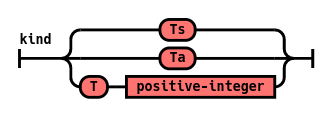
\includegraphics{nstar-kinds-syntax}
  }
  \caption{Grammar for kinds.}
  \label{fig:nstar-common-ts-kinds-syntax}
\end{figure}

\subsection{Integer types}\label{subsec:nstar-common-ts-integer}

Numbers are the building block of any assembly language. Most of data manipulated is manipulated as numbers, e.g.\ addresses, characters, strings, enumerations, etc.
This is not the case in N*, where ``integer''  only really means ``number''.
The syntax for the types of integers is given in Figure~\ref{fig:nstar-common-ts-integer-syntax}.

\begin{figure}[htb]
  \centering
  \scalebox{.5}{
    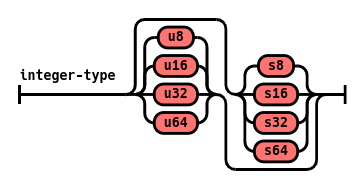
\includegraphics{nstar-integers-types-syntax}
  }
  \caption{Grammar for integer types.}
  \label{fig:nstar-common-ts-integer-syntax}
\end{figure}

Integers have two varying parameters: their sign and sizes.
According to the sign (i.e.\ signed or unsigned), some operations may not perform the same (for example \texttt{mul} does not behave the same).
The size is nothing more than the number of bits occupied by the integer (in N*, those are restricted to multiples of $8$ smaller or equal to $64$).
Most operations should perform the same no matter the integer size, however it is recommended to search in the target architecture manual for further reference.

Kinds of integers are written under the form of inference rules in Figure~\ref{fig:nstar-common-ts-integer-kindrules}.

\begin{figure}[htb]
  \centering

  \begin{prooftree}
    \Infer0{\Gamma\Vdash$ u64 : T8$}
  \end{prooftree}
  \hspace{3em}
  \begin{prooftree}
    \Infer0{\Gamma\Vdash$ s64 : T8$}
  \end{prooftree}
  \hspace{3em}
  \begin{prooftree}
    \Infer0{\Gamma\Vdash$ u32 : T4$}
  \end{prooftree}
  \hspace{3em}
  \begin{prooftree}
    \Infer0{\Gamma\Vdash$ s32 : T4$}
  \end{prooftree}
  \\\vspace{\baselineskip}
  \begin{prooftree}
    \Infer0{\Gamma\Vdash$ u16 : T2$}
  \end{prooftree}
  \hspace{3em}
  \begin{prooftree}
    \Infer0{\Gamma\Vdash$ s16 : T2$}
  \end{prooftree}
  \hspace{3em}
  \begin{prooftree}
    \Infer0{\Gamma\Vdash$ u8 : T1$}
  \end{prooftree}
  \hspace{3em}
  \begin{prooftree}
    \Infer0{\Gamma\Vdash$ s8 : T1$}
  \end{prooftree}

  \caption{Kind inference rules for integers.}
  \label{fig:nstar-common-ts-integer-kindrules}
\end{figure}

\subsection{Other atomic types}\label{subsec:nstar-common-ts-otheratomic}

There are two other atomic types that we did not talk about, but refered to in the introduction of the type system: characters and pointers. Their respective syntax is given in Figure~\ref{fig:nstar-common-ts-atomic-syntax}.

\begin{figure}[htb]
  \centering
  \scalebox{.5}{
    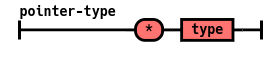
\includegraphics{nstar-ptr-type-syntax}
  } \\
  \scalebox{.5}{
    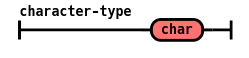
\includegraphics{nstar-char-type-syntax}
  }
  \caption{Grammar for character and pointer types}
  \label{fig:nstar-common-ts-atomic-syntax}
\end{figure}

In all assembly languages, characters are merely syntactic sugar for their ASCII code. This is how their are put in the machine code anyway, so it is not a huge problem (it might even not be at all).

Pointers, on the other hand, are unabstracted memory addresses.
In N*, there are two types of pointers: data pointers and stack pointers.
Stack pointers are covered in Subsection~\ref{subsec:nstar-common-ts-stack}~``\nameref{subsec:nstar-common-ts-stack}''.
Data pointers simply represent an address where we know (or not, see the Subsection~\ref{subsec:nstar-common-unsafe-derefliteraladdr}~``\nameref{subsec:nstar-common-unsafe-derefliteraladdr}'') that there is a value of the given pointed type.

Kind inference is given in Figure~\ref{fig:nstar-common-ts-atomic-kindrules}.

They support two common operations: offsetting (see the Subsection~\ref{subsec:nstar-common-unsafe-ptroffset}~``\nameref{subsec:nstar-common-unsafe-ptroffset}'') and dereferencing (taking the value pointed by the pointer).
Dereferencing is considered a safe operation, unless trying to on a literal address.
There is no notion of ``null'' pointers, like \texttt{NULL} in C.
However, it is possible to use the literal \texttt{\$0} (which represents a pointer to the address $0$).

\begin{figure}[htb]
  \centering
  \begin{prooftree}
    \Infer0{\Gamma\Vdash$ char : T1$}
  \end{prooftree}
  \hspace{3em}
  \begin{prooftree}
    \Hypo{\Gamma\Vdash$ t : Ta$}
    \Infer1[64-bits pointers]{\Gamma\Vdash$ *t : T8$}
  \end{prooftree}
  \hspace{3em}
  \begin{prooftree}
    \Hypo{\Gamma\Vdash$ t : Ta$}
    \Infer1[32-bits pointers]{\Gamma\Vdash$ *t : T4$}
  \end{prooftree}

  \caption{Kind inference rules for other atomic types.}
  \label{fig:nstar-common-ts-atomic-kindrules}
\end{figure}

\subsection{Context types}\label{subsec:nstar-common-ts-records}

Record types (or contexts) are mappings from registers to types.
They are used to indicate that a register is bound to a value of a given type at a certain point in the program.
The grammar is described in Figure~\ref{fig:nstar-common-ts-records-syntax}.

\begin{figure}[htb]
  \centering
  \scalebox{.5}{
    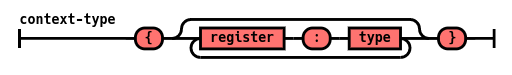
\includegraphics{nstar-records-syntax}
  }
  \caption{Grammar for context types.}
  \label{fig:nstar-common-ts-records-syntax}
\end{figure}

Context types are used to represent data contexts where any mapping is some sort of a proof that some data of some type is accessible through some register.

\vspace{\baselineskip}

\textbf{Note:} In the context of label types, a context type can be augmented by a \texttt{forall} generic type variable binder.
The grammar is described in Figure~\ref{fig:nstar-common-ts-label-types-syntax}.
The type variable binder is used to abstract away some details of the type through an opaque variable specialized at the call site.

\begin{figure}[htb]
  \centering
  \scalebox{.5}{
    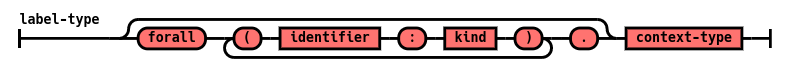
\includegraphics{nstar-label-types-syntax}
  }
  \caption{Grammar for label context types.}
  \label{fig:nstar-common-ts-label-types-syntax}
\end{figure}

The example code given in Listing~\ref{lst:nstar-common-ts-records-stackmask} shows a use for type variables.
The stack is abstracted away, meaning that we can call this function from anywhere, given any stack (as long as it is \texttt{call}ed, or \texttt{jmp}ed to from a \texttt{call}ed function).
The type variable \texttt{s} is specialized at the call site.

\begin{listing}[htb]
  \centering
  \begin{minipage}{0.90\textwidth}
    \begin{minted}[]{\nstarlexer}
      label: forall (s: Ts). { %rsp: sptr *{ %rsp: sptr s }::s }
          ret
    \end{minted}
  \end{minipage}
  \caption{Stack masking using a type variable binder.}
  \label{lst:nstar-common-ts-records-stackmask}
\end{listing}

\subsection{Stack types}\label{subsec:nstar-common-ts-stack}

There are mainly two stack types in N*: the stack pointer \texttt{sptr} and the stack constructor \texttt{::}.
Note that there is no ``empty stack'' type as would be the case with e.g.\ lists in Haskell.
The reason is that it forces the developer to abstract the stack to be able to have a ``stack tail'' (the part of the stack on the right of the stack constructor \texttt{::}) at some point.\footnote{It also serves the purpose to ensure that we cannot construct a stack from nothing, and that it should always be given to us, to e.g.\ the \texttt{main} function.}
An example is given in Listing~\ref{lst:nstar-common-ts-records-stackmask}.

The grammar for stack types is given in Figure~\ref{fig:nstar-common-ts-stack-types-syntax}.

Inference rules for kinds of stack types are written in Figure~\ref{fig:nstar-common-ts-stack-types-kindrules}

\begin{figure}[htb]
  \centering
  \scalebox{.5}{
    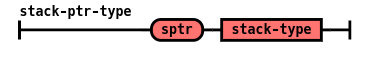
\includegraphics{nstar-stack-pointer-syntax}
  }
  \\
  \scalebox{.5}{
    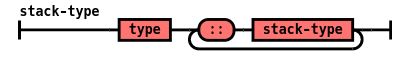
\includegraphics{nstar-stack-cons-syntax}
  }
  \caption{Grammar for stack types.}
  \label{fig:nstar-common-ts-stack-types-syntax}
\end{figure}

\begin{figure}[htb]
  \centering

  \begin{prooftree}
    \Hypo{\Gamma\Vdash$ s : Ts$}
    \Infer1[32-bits pointers]{\Gamma\Vdash$ sptr s : T4$}
  \end{prooftree}
  \hspace{3em}
  \begin{prooftree}
    \Hypo{\Gamma\Vdash$ s : Ts$}
    \Infer1[64-bits pointers]{\Gamma\Vdash$ sptr s : T8$}
  \end{prooftree}
  \\\vspace{\baselineskip}
  \begin{prooftree}
    \Hypo{$n : $\mathbb{N}$ $}
    \Hypo{\Gamma\Vdash$ t : Tn$}
    \Hypo{\Gamma\Vdash$ s : Ts$}
    \Infer3{\Gamma\Vdash$ t :: s : Ts$}
  \end{prooftree}

  \caption{Kind inference rules for stack types}
  \label{fig:nstar-common-ts-stack-types-kindrules}
\end{figure}

\subsection{Structure types}\label{subsec:nstar-common-ts-structs}

Structure types are packed sets of unnamed types (compared to context types, each field does not have a name, only a type) that can be indexed from a pointer only to a full field (so if you have two \texttt{u64}s, you can only offset to $0$ and $8$, respectively for the first and second field).

Grammar is described in Figure~\ref{fig:nstar-common-ts-structs-syntax} and kind inference rules are given in Figure~\ref{fig:nstar-common-ts-structs-kindrules}.

Structures take as much space as all their fields, thus can mainly be put on the stack (unless being less than 8 bytes, which is the upper limit for register sizes in current architectures).

\begin{figure}[htb]
  \centering
  \scalebox{.5}{
    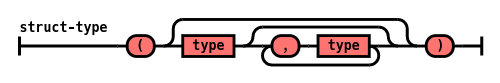
\includegraphics{nstar-struct-types-syntax}
  }

  \caption{Grammar for structure types.}
  \label{fig:nstar-common-ts-structs-syntax}
\end{figure}

\begin{figure}[htb]
  \centering
  \begin{prooftree}
    \Hypo{$n$_0$, n$_1$, $\ldots$, n$_p$ : $\mathbb{N}}
    \Hypo{\Gamma\Vdash$ t$_0$ : Tn$_0$, t$_1$ : Tn$_1$, $\ldots$, t$_p$ : Tn$_p}
    \Hypo{$m = $\sum_{i = 0}^{p}{n_i}}
    \Infer3{\Gamma\Vdash$ (t$_0$, t$_1$, $\ldots$, t$_p$) : Tm$}
  \end{prooftree}

  \caption{Kind inference rule for structures.}
  \label{fig:nstar-common-ts-structs-kindrules}
\end{figure}

\subsection{Union types}\label{subsec:nstar-common-ts-unions}

Union types simply are overlapping data bits, which can be given meaning depending on what type you decide to access.
Grammar for union types is given in Figure~\ref{fig:nstar-common-ts-unions-syntax}.

\begin{figure}[htb]
  \centering
  \scalebox{.5}{
    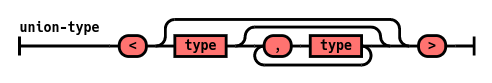
\includegraphics{nstar-union-types-syntax}
  }

  \caption{Grammar for union types.}
  \label{fig:nstar-common-ts-unions-syntax}
\end{figure}

Unions are sized depending on the types they unite: their sizes will be the maximum of all the sizes of all the components.
This is more clear in the kind inference rule given in Figure~\ref{fig:nstar-common-ts-unions-kindrules}.

\begin{figure}[htb]
  \centering

  \begin{prooftree}
    \Hypo{$n$_0$, n$_1$, $\ldots$, n$_p$ : $\mathbb{N}}
    \Hypo{\Gamma\Vdash$ t$_0$ : n$_0$, t$_1$ : n$_1$, $\ldots$, t$_p$ : n$_p}
    \Hypo{$m = $\max_{i = 0}^{p}{n_i}}
    \Infer3{\Gamma\Vdash$ $\langle$t$_0$, t$_1$, $\ldots$, t$_p\rangle$ : Tm$}
  \end{prooftree}

  \caption{Kind inference rules for union types.}
  \label{fig:nstar-common-ts-unions-kindrules}
\end{figure}

Note that unlike structure types, you will most likely be storing union types in registers, unless working with very big unions.
Also, accessing a union's field is considered an unsafe operation, but this will be more detailed in another section on expressions.

\section{File sections}\label{sec:nstar-common-sections}

Sections in N* serve the exact same purpose as in other assembly languages. They divide a file into multiple parts depending on what the semantics of the current section is supposed to be (code, data, etc).
Section names obviously differ from one target format to another. As an example, the ``\texttt{.rela.dyn}'' section from the ELF format may not exist in the PE format.

N* tries to unify target formats section names (simplifying targetting N* as a compiler backend) by having a fixed set of section names, all with different meanings. While you can put anything anywhere in classical assembly languages, this is not the case in N*.

Sections in N* can be named ``\texttt{data}'', ``\texttt{code}'', ``\texttt{rodata}'', ``\texttt{udata}'' or ``\texttt{extern}''. Each of them has defined semantics as described below.

\subsection{The \texttt{code} section}\label{subsec:nstar-common-sections-code}

The \texttt{code} section is the section containing all executable instructions (basically, as the name implies, code).
Its syntax is defined in Figure~\ref{fig:nstar-common-sections-code-grammar}.

Each label is assigned a type, describing the context needed to branch to it.
If a label has the type \texttt{\{reg:s64\}} then there needs to be the register \texttt{reg} bound to a value of type \texttt{s64} in the current context, in order to branch to it.
However, some restrictions apply to labels in order to make the type-checking meaningful (or at least handle some aspects that cannot be handled with types only). See more about that in Section~\ref{sec:nstar-common-bs}~``\nameref{sec:nstar-common-bs}''.

\begin{figure}[htb]
  \centering
  \scalebox{.5}{
    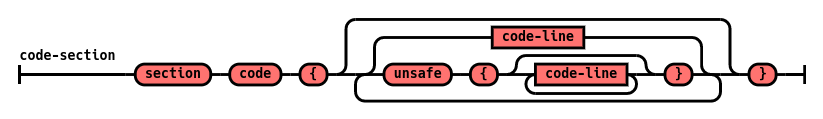
\includegraphics{nstar-code-section-1}
  }
  \\
  \scalebox{.5}{
    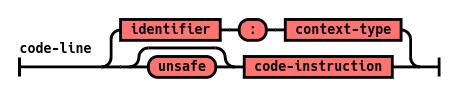
\includegraphics{nstar-code-section-2}
  }

  \caption{Grammar for \texttt{code} sections.}
  \label{fig:nstar-common-sections-code-grammar}
\end{figure}

Every assembly instruction makes the current context vary in some way, either by binding registers, forgetting about some bindings, changing register types, or some other way. The current context is just a record keeping track of the currently bound registers, along with the data type they contain.
More on that in sections about instructions\footnote{Instructions are platform-specific, that's why we don't talk about them here.}.

\subsection{The \texttt{data}, \texttt{rodata} and \texttt{udata} sections}\label{subsec:nstar-common-sections-data}

The \texttt{data} and \texttt{rodata} sections are sections used to reference (read-only) literal data (much like constants in PHP).
Each label in those sections is used as a pointer to the given value, but only the labels in the \texttt{data} section can be written to\footnote{The \texttt{rodata} section (read-only data) is read-only. While it is not necessary to prevent writing to it at compile-time, it is an undefined behavior at runtime.}.
The grammar of those sections is given in Figure~\ref{fig:nstar-common-sections-data-grammar}.

\begin{figure}[htb]
  \centering
  \scalebox{.5}{
    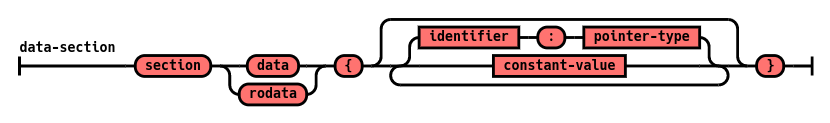
\includegraphics{nstar-data-section-grammar}
  }

  \caption{Grammar for the \texttt{data}, \texttt{rodata} and \texttt{udata} sections.}
  \label{fig:nstar-common-sections-data-grammar}
\end{figure}

\noindent Note that, while the grammar allows labels in the \texttt{data} section to be pointers to context types, this cannot be typed because there is no such constant value referencing a code-space address.

While the \texttt{data} and \texttt{rodata} sections contain initialised values (that is, hardcoded bytes in the executable), the \texttt{udata} section does not contain any byte (it should be only $0$s, to reserve space for each entry).

\subsection{The \texttt{extern} sections}\label{subsec:nstar-common-sections-extern}

The \texttt{extern} sections contain information related to static and dynamic imports.
They come in 2 flavors: function imports or data imports.

\subsubsection{The \texttt{extern.code} section}\label{subsubsec:nstar-common-sections-extern-code}

The \texttt{extern.code} section indicates that there are functions which, despite not being in the source file, should be accessible with the given context.
Static imports are resolved during linking, preventing from using undefined function symbols at runtime, while dynamic imports are resolved at runtime by the dynamic linker.
The two types of imports are indicated from the absence (or presence) of the \texttt{dyn} qualifier when importing.
The grammar showing this is given in figure~\ref{fig:nstar-common-sections-extern-code-grammar}.

\begin{figure}[htb]
  \centering
  \scalebox{.47}{
    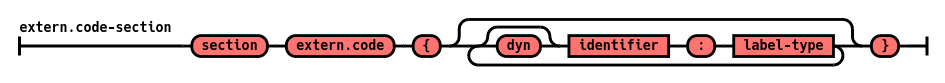
\includegraphics{nstar-externcode-section-grammar}
  }

  \caption{Grammar for the \texttt{extern.code} file section.}
  \label{fig:nstar-common-sections-extern-code-grammar}
\end{figure}

\subsubsection{The \texttt{extern.data} and \texttt{extern.rodata} sections}\label{subsubsec:nstar-common-sections-extern-data}

The \texttt{extern.data} and \texttt{extern.rodata} sections are used to import data addresses into the current scope.
While it is possible to dynamically import a data address, it shouldn't really be useful (unless in specific cases like \texttt{static} variables).
Same as for the \texttt{extern.code} section, the import type (dynamic or static) is given depending on the absence (or presence) of the \texttt{dyn} qualifier.
The grammar for this section is given in Figure~\ref{fig:nstar-common-sections-extern-data-grammar}.

\begin{figure}[htb]
  \centering
  \scalebox{.45}{
    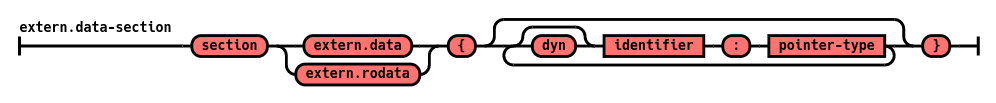
\includegraphics{nstar-externdata-section-grammar}
  }

  \caption{Grammar for the \texttt{extern.data} and \texttt{extern.rodata} sections.}
  \label{fig:nstar-common-sections-extern-data-grammar}
\end{figure}

\section{Constant values}\label{sec:nstar-common-constvalue}

Constant values are some kind of values that can be used in the \texttt{data} and \texttt{rodata} sections\footnote{See Section~\ref{subsec:nstar-common-sections-data}~``\nameref{subsec:nstar-common-sections-data}''.}.
They come in 3 flavors: integers, characters and arrays.
Their grammar is given in Figure~\ref{fig:nstar-common-constvalue-grammar} and the type inference rules are given in Figure~\ref{fig:nstar-common-constvalue-typerules}.

\begin{figure}[htb]
  \centering
  \scalebox{.5}{
    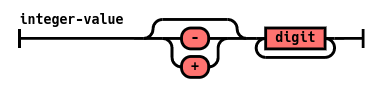
\includegraphics{nstar-integer-grammar}
  }
  \\
  \scalebox{.5}{
    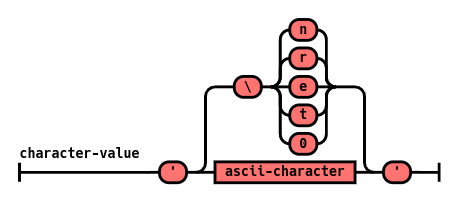
\includegraphics{nstar-character-grammar}
  }
  \\
  \scalebox{.5}{
    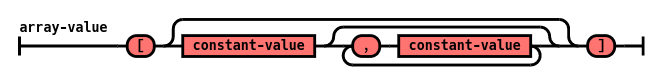
\includegraphics{nstar-array-grammar}
  }

  \caption{Grammar for constant values.}
  \label{fig:nstar-common-constvalue-grammar}
\end{figure}

\begin{figure}[htb]
  \centering

  \begin{prooftree}
    \Hypo{$d is a signed integer constant$}
    \Hypo{$t $\in\{$s8, s16, s32, s64$\}}
    \Infer2{\vdash_{data}$ d : t$}
  \end{prooftree}
  \\\vspace{\baselineskip}
  \begin{prooftree}
    \Hypo{$d is an unsigned integer constant$}
    \Hypo{$t $\in\{$u8, u16, u32, u64$\}}
    \Infer2{\vdash_{data}$ d : t$}
  \end{prooftree}
  \\\vspace{\baselineskip}
  \begin{prooftree}
    \Hypo{$c is a character constant$}
    \Infer1{\vdash_{data}$ c : char$}
  \end{prooftree}
  \\\vspace{\baselineskip}
  \begin{prooftree}
    \Hypo{$n : $\mathbb{N}}
    \Hypo{\Gamma\Vdash$ t : Tn$}
    \Hypo{\vdash_{data}$ c$_1$, c$_2$, \ldots, c$_n$ : t$}
    \Infer3{\vdash_{data}$ [c$_1$, c$_2$, \ldots, c$_n$] : *t$}
  \end{prooftree}

  \caption{Type inference rules for constant values.}
  \label{fig:nstar-common-constvalue-typerules}
\end{figure}

\section{Restrictions applied to branching}\label{sec:nstar-common-bs}

Branching ((un-)\ conditional jumps, calls, etc) is restricted in N* in order to prevent stack leaks, unknown caller address return or even missing return values.
It also is restricted not to integrate some sort of scoping, which would add some (mostly useless) complexity when using/generating N*.

\subsection{Returning to a known code-space address}\label{subsec:nstar-common-bs-ret}

Because the stack is given a type in N*, we can use it to make sure that we are returning to a code-space address.
When we \texttt{call} a label, we are pushing the current instruction pointer on top of the stack (the stack pointer is \texttt{\%rip} on x86/x64, \texttt{\$ip} on MIPS, etc) before jumping to the callee address.

Because of that, the type given to the stack for the context of a label contains at least a pointer to some context (\texttt{*\{ binds\ldots\ \}}) on the very top of it (unless this label is never meant to be \texttt{call}ed but rather \texttt{jmp}ed to).
This is later used by \texttt{ret} in order to determine that returning from this function can be done safely, and \textit{should}\footnote{It should return to a valid address, but this cannot be checked nor endorsed when using, for example, the foreign function interface or when creating a \texttt{main} function.} return to a valid code-space address.
If any other data-type is present on top of the stack (an integer, a pointer to something else than a context, a stack pointer, a structure, an union), \texttt{ret} \textit{must} fail to type-check, preserving the stack at runtime and preventing an undefined behavior.

\subsection{Missing return values (a.k.a.\ registers not bound before return)}\label{subsec:nstar-common-bs-unboundregs}

Along with checking that we are returning to a valid code-space address, we can also, thanks to the type of the stack, determine if returning from a function preserves the value in registers, and if after returning we have access to return values of a function.
Consider the example given in Listing~\ref{lst:nstar-common-bs-returnvalues}.

When \texttt{ret}urning from the \texttt{example} ``function'', we give access to the values of type \texttt{u64} in the \texttt{\%rax} and \texttt{\%rbx} registers.
Note that if either of those registers were not bound before (not given as parameters, or bound using \texttt{mov}), type-checking \textit{must} fail to prevent undefined behavior when later accessing the ``value'' in either register.
We can easily see that the return context contains \texttt{\%rax: u64} and \texttt{\%rbx: u64}, which means that both registers must have been bound before, and are accessible for reading later one, after the \texttt{call} that went until here.
This gives a safe way of using return values, and guaranteeing that there are indeed return values stored in the target registers.

\begin{listing}[htb]
  \centering
  \begin{minipage}{0.90\textwidth}
    \begin{minted}[]{\nstarlexer}
    example: forall (s: Ts). { %rsp: sptr *{ %rsp: sptr s, %rax: u64, %rbx: u64 } }
      mov 0, %rax
      mov 5, %rbx
      ret
    \end{minted}
  \end{minipage}
  \caption{An example of returning multiple values from a simple function.}
  \label{lst:nstar-common-bs-returnvalues}
\end{listing}

\subsection{Type-checking and scoping problems}\label{subsec:nstar-common-bs-tcscopes}

The type system in N* cannot detect control flow leaks.
One common idiom in assembly languages is the possibility of doing things like in Listing~\ref{lst:nstar-common-bs-labeljumping}.
The idea is pretty simple: a label is just a way of naming a code-space address (or data-space address, but it is not the main concern here) which points to the next instruction after it.
This works in plain assembly languages because of the lack of an advanced type system like the one N* has.

\begin{listing}[htb]
  \centering
  \begin{minipage}{0.90\textwidth}
    \begin{minted}[]{asm}
    f:
      cmp %rax, $0
      je r
    tmp:
      mov $0, %rax
    r:
      ret
    \end{minted}
  \end{minipage}
  \caption{A simple case of jumping through a label (here \texttt{tmp}) in the GNU Assembler.}
  \label{lst:nstar-common-bs-labeljumping}
\end{listing}

In N*, however, because you must specify the branching context of a label, jumping through one cannot be allowed without some sort of scoping notion.
Take the example in Listing~\ref{lst:nstar-common-bs-labeljumping2}.
The instruction \texttt{jmp tmp<s>} seems unneeded (in fact, it can be optimized away), but it really is to ensure type-checking is correct, as per N*'s semantics.

\begin{listing}[htb]
  \centering
  \begin{minipage}{0.90\textwidth}
    \begin{minted}[]{\nstarlexer}
      f: forall (s: Ts). { %rsp: sptr *{ %rsp: sptr s, %rax: u64 }::s, %rax: u64 }
        cmp %rax, 0
        je r<s>
        jmp tmp<s>
      tmp: forall (s: Ts). { %rsp: sptr *{ %rsp: sptr s, %rax: u64 }::s, %rax: u64 }
        mov 0, %rax
        jmp r<s>
      r: forall (s: Ts). { %rsp: sptr *{ %rsp: sptr s, %rax: u64 }::s, %rax: u64 }
        ret
    \end{minted}
  \end{minipage}
  \caption{The same example as Listing~\ref{lst:nstar-common-bs-labeljumping}, but in N*.}
  \label{lst:nstar-common-bs-labeljumping2}
\end{listing}

Trying to remove this instruction makes us question about type-checking: what solution do we have when type-checking the \texttt{tmp} label? (same reasoning can be applied for the \texttt{r} label)
\begin{itemize}
  \item
        One way would be to try to unify \texttt{tmp}'s context type with the current context.
        While this works for this specific example, there are plenty of examples where this would not work, for example trying to type-check \texttt{f} this way (which basically would fail because the current context is empty).

        Also, how would we infer that the \texttt{s} stack type used in \texttt{tmp}'s type is the same as the one used in \texttt{f}'s type?
        Going by name isn't the way, as we might want to do \texttt{jump tmp<sss>} (where \texttt{sss} is bound in \texttt{f}'s context but not \texttt{tmp}'s context).
  \item
        Another way is to introduce scopes, where \texttt{tmp} becomes a ``sub-label'' of \texttt{f}, being allowed to now use the rigid type variable \texttt{s} bound in its parent's context.
        This obviously seems to work, but introduces quite a lot of complexity in the making of the code, for example how do we introduce a new block (indentation-based? with \texttt{\{\}}?), what are the semantics, will the syntax clash with types, etc.

        This however solves the type variable specialization problem, but still leaves the type-checking of child labels unresolved.
\end{itemize}

Branch-checking is therefore used to guarantee that every label is branched to at some point in time, and that the control flow never leaks through a label.

\section{Unsafe operations}\label{sec:nstar-common-unsafe}

Unsafe operations are operations (sequence of zero or more instructions) whose safety cannot be determined from the current context, or whose evaluation cannot be determined as not UB-provoking (that is, the evaluation may put the application in an unknown state).
Those kind of operations are essential to low-level programming, but we want to put an emphasis on them by separating them from the rest of the normal and safe operations using \texttt{unsafe} blocks.

\subsection{Dereferencing literal addresses}\label{subsec:nstar-common-unsafe-derefliteraladdr}

Sometimes, one needs to be able to read from/write to literal addresses, such as \texttt{0xB8000} in kernel development (this is the console text buffer beginning address, used to output text to the basic 80×25 console).
However, because you cannot guarantee that 1- the memory address exists on every machine the program is supposed to run on and 2- there always are some reconstitutable pieces of data of the specified type at the given address, those two operations are considered unsafe.
Be aware that, despite not being restricted, trying to write to a protected memory address yields an undefined behavior.
Also, if used, the code is no-longer considered platform-independendant\footnote{Platform independant code (PIC for short) is a type of code which should be runnable on all machines, no matter their specifications.}.

\subsection{Pointer offsetting}\label{subsec:nstar-common-unsafe-ptroffset}

Stack pointers, because of their type, can be safely offset to point to a valid piece of data.
However, ``normal'' pointers (for example \texttt{*u64}) cannot be safely offset.
While a stack pointers describes the entire structure of the stack (or at least a piece of it), a regular pointer only describes the piece of data it points to.

This is a common idiom in C to use pointers to represent arrays in a contiguous memory (so an array of 6 integers would basically be a $6 * sizeof(int)$ bytes wide chunk of memory, where each index points to a different integer).
\texttt{Vec<T>} in Rust, \texttt{std::vector<T>} in C++, \texttt{ArrayList<T>} in Java, and many other vector types are also implemented in terms of a pointer to a chunk of memory, but with an added container size, allowing to safely access elements of the vector without going out of bounds.
But in Rust, we still need to have some \texttt{unsafe} blocks in your code, in order to use the container.

There is the same problem in N*.
Because there is no built-in array type, we have to rely on pointers to be able to achieve such thing, therefore needing a way to offset a pointer to access the various elements in the array.
It would also be really hard to manipulate plain array types (because, for example, of the size to store with the type).
As offsetting a pointer can lead to an invalid address dereferencing (or at least dereferencing an address which doesn't belong to the application memory, i.e.\ allocated by another process), it is considered an unsafe operation and therefore needs to be wrapped in an \texttt{unsafe} block.

\chapter{Instructions and target-dependent features}\label{chap:nstar-specific}

\section{Introduction}\label{sec:nstar-specific-introduction}

In addition to the special notation for inference rules introduced in the precedent chapter\footnote{See Section~\ref{sec:nstar-common-introduction}~``\nameref{sec:nstar-common-introduction}''}, there is:
\begin{itemize}
  \item $\vdash_{code}$, describing the inference process in a \texttt{code} section;
  \item $\Delta$, which is the current typing environment (associating registers with the type of data they hold);
\end{itemize}

\section{x86, amd64}\label{sec:nstar-specific-x86amd64}

\subsection{Available registers}\label{subsec:nstar-specific-x86amd64-registers}

\begin{tabularx}{\textwidth}{*{8}{| >{\centering\arraybackslash}X} |}
  \hline
  \textbf{64} & \textbf{56} & \textbf{48} & \textbf{40} & \textbf{32} & \textbf{24} & \textbf{16} & \textbf{8} \\
  \hline

  \rowcolor{gray!30}%
  \multicolumn{8}{|c|}{\textbf{General purpose registers: A, B, C and D}} \\
  \hline

  \multicolumn{8}{|c|}{R?X} \\
  \hline
  \multicolumn{4}{|c|}{\cellcolor{gray!10}} & \multicolumn{4}{c|}{E?X} \\
  \hline
  \multicolumn{6}{|c|}{\cellcolor{gray!10}} & \multicolumn{2}{c|}{?X} \\
  \hline
  \multicolumn{6}{|c|}{\cellcolor{gray!10}} & {?H} & {?L} \\
  \hline

  \rowcolor{gray!30}%
  \multicolumn{8}{|c|}{\textbf{Index registers: S and D}} \\
  \hline

  \multicolumn{8}{|c|}{R?I} \\
  \hline
  \multicolumn{4}{|c|}{\cellcolor{gray!10}} & \multicolumn{4}{c|}{E?I} \\
  \hline
  \multicolumn{6}{|c|}{\cellcolor{gray!10}} & \multicolumn{2}{c|}{?I} \\
  \hline
  \multicolumn{7}{|c|}{\cellcolor{gray!10}} & {?IL} \\
  \hline

  \rowcolor{gray!30}%
  \multicolumn{8}{|c|}{\textbf{Pointer registers: S and B\makebox[0pt][l]{$^{\ast}$} }} \\
  \hline

  \multicolumn{8}{|c|}{R?P} \\
  \hline
  \multicolumn{4}{|c|}{\cellcolor{gray!10}} & \multicolumn{4}{c|}{E?P} \\
  \hline

  \hline
  \multicolumn{8}{|l|}{\textit{\footnotesize$^{\ast}$ RSP and RBP are only available in 64-bit mode, while ESP and EBP are only available in 32-bit mode.}} \\
  \hline
\end{tabularx}

\subsection{Expressions}\label{subsec:nstar-specific-x86amd64-exprs}

There are four types of expressions in x86-N*: immediate values, data labels, registers and pointer offsets.
All of these can be used as the value operand of the \texttt{mov} instruction.

\subsubsection{Immediate values}\label{subsubsec:nstar-specific-x86amd64-exprs-immediate}

Immediate values are also known as ``hardcoded values''.
These are values that you can directly read in the source file, and which do not come from e.g.\ registers.
Grammar and inference rules are given respectively in Figure~\ref{fig:nstar-specific-x86amd64-exprs-immediate-grammar} and Figure~\ref{fig:nstar-specific-x86amd64-exprs-immediate-typerules}.

\begin{figure}[htb]
  \centering
  \scalebox{.5}{
    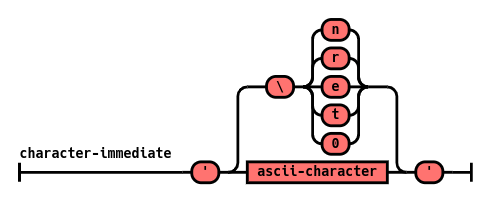
\includegraphics{nstar-imm-char-grammar}
  }
  \\
  \scalebox{.5}{
    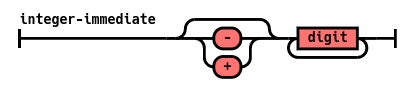
\includegraphics{nstar-imm-int-grammar}
  }
  \caption{Grammar for immediate values in x86-N*.}
  \label{fig:nstar-specific-x86amd64-exprs-immediate-grammar}
\end{figure}

\begin{figure}[htb]
  \centering

  \begin{prooftree}
    \Hypo{$c is a character immediate$}
    \Infer1{\Delta\vdash_{code}$ c : char$}
  \end{prooftree}
  \\\vspace{\baselineskip}
  \begin{prooftree}
    \Hypo{$i is an unsigned integer immediate$}
    \Hypo{$t $\in\{$ u8, u16, u32, u64 $\}}
    \Infer2{\Delta\vdash_{code}$ i : t$}
  \end{prooftree}
  \\\vspace{\baselineskip}
  \begin{prooftree}
    \Hypo{$i is a signed integer immediate$}
    \Hypo{$t $\in\{$ s8, s16, s32, s64 $\}}
    \Infer2{\Delta\vdash_{code}$ i : t$}
  \end{prooftree}

  \caption{Type inference rules for immediate values in x86-N*.}
  \label{fig:nstar-specific-x86amd64-exprs-immediate-typerules}
\end{figure}

\subsubsection{Data labels}\label{subsubsec:nstar-specific-x86amd64-exprs-labels}

Data labels are pointers to some piece of data (may it even be an array).
They can be dereferenced and offset using the constructs given in N*.
Grammar and inference rules are given respectively in Figure~\ref{fig:nstar-specific-x86amd64-exprs-labels-grammar} and Figure~\ref{fig:nstar-specific-x86amd64-exprs-labels-typerules}.

\begin{figure}[htb]
  \centering

  \scalebox{.5}{
    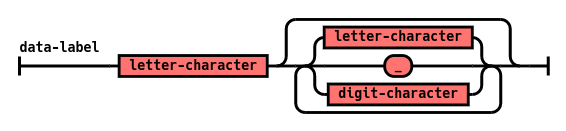
\includegraphics{nstar-label-expr-grammar}
  }
  \caption{Grammar for data labels in x86-N*.}
  \label{fig:nstar-specific-x86amd64-exprs-labels-grammar}
\end{figure}

\begin{figure}[htb]
  \centering

  \begin{prooftree}
    \Hypo{$x is a known label$}
    \Hypo{\vdash_{data}$ x : *t$}
    \Infer2{\Delta\vdash_{code}$ x : *t$}
  \end{prooftree}

  \caption{Type inference rules for data labels in x86-N*.}
  \label{fig:nstar-specific-x86amd64-exprs-labels-typerules}
\end{figure}

\subsubsection{Registers}\label{subsubsec:nstar-specific-x86amd64-exprs-registers}

Registers are basically value containers.
They can also be dereferenced and offset (applying those operations to the contained value).
Grammar is given in Figure~\ref{fig:nstar-specific-x86amd64-exprs-registers-grammar} and type inference rules are given in Figure~\ref{fig:nstar-specific-x86amd64-exprs-registers-typerules}.

\begin{figure}[htb]
  \centering

  \scalebox{.5}{
    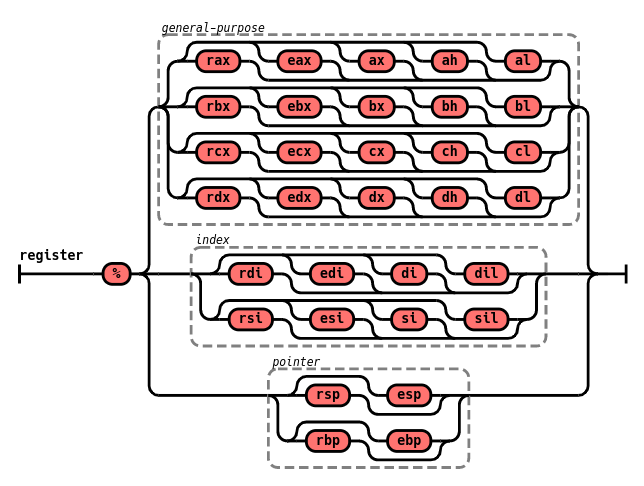
\includegraphics{nstar-register-x86-grammar}
  }
  \caption{Grammar for registers in x86-N*.}
  \label{fig:nstar-specific-x86amd64-exprs-registers-grammar}
\end{figure}

\begin{figure}[htb]
  \centering

  \begin{prooftree}
    \Hypo{$r is a register$}
    \Infer1{\Delta$, r : t $\vdash_{code}$ r : t$}
  \end{prooftree}

  \caption{Inference rules for register values.}
  \label{fig:nstar-specific-x86amd64-exprs-registers-typerules}
\end{figure}

\subsubsection{Pointer offsets}\label{fig:nstar-specific-x86amd64-exprs-pointeroffsets}

Pointer offsets allow accessing data that may be located relative to a given memory address.
Grammar for pointer offsets is given in Figure~\ref{fig:nstar-specific-x86amd64-exprs-pointeroffsets-grammar} and type inference rules are given in Figure~\ref{fig:nstar-specific-x86amd64-exprs-pointeroffsets-typerules}.

\begin{figure}[htb]
  \centering

  \scalebox{.5}{
    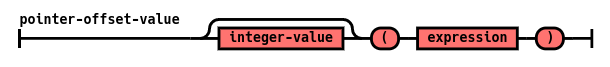
\includegraphics{nstar-pointer-offset-grammar}
  }

  \caption{Grammar for pointer offsets.}
  \label{fig:nstar-specific-x86amd64-exprs-pointeroffsets-grammar}
\end{figure}

\begin{figure}[htb]
  \centering

  \begin{prooftree}
    \Hypo{$n$_1$, n$_2$, \ldots, n$_p$ $\in\mathbb{N}}
    \Hypo{$m$_i$ = $-$n$_i}
    \Infer[no rule, rule margin=1.0ex]2{\Gamma\Vdash$ t$_1$ : Tn$_1$, t$_2$ : Tn$_2$, \ldots, t$_p$ : Tn$_p$, s : Ts\hspace{1.5em}$%
                                        \Delta\vdash_{code}$ e : sptr t$_1$::t$_2$::\ldots::t$_p$::s$}
    \Infer1[Stack pointers]{\Delta\vdash_{code}$ m$_i$(e) : t$_i}
    % small hack: makes all premises on top of each other
  \end{prooftree}
  \\\vspace{\baselineskip}
  \begin{prooftree}
    \Hypo{$n$_1$, n$_2$, \ldots, n$_p$ $\in\mathbb{N}}
    \Infer[no rule, rule margin=1.0ex]1{\Gamma\Vdash$ t$_1$ : Tn$_1$, t$_2$ : Tn$_2$, \ldots, t$_p$ : Tn$_p$\hspace{1.5em}$%
                                        \Delta\vdash_{code}$ e : *$ ($ t$_1$::t$_2$::\ldots::t$_p$ $)}
    \Infer1[Structure pointers]{\Delta\vdash_{code}$ n$_i$(e) : t$_i}
    % small hack: makes all premises on top of each other
  \end{prooftree}
  \\\vspace{\baselineskip}
  \begin{prooftree}
    \Hypo{$k, n $\in\mathbb{N}}
    \Hypo{$m = k $\times$ n$}
    \Hypo{\Gamma\Vdash$ t : Tn$}
    \Hypo{\Delta\vdash_{code}$ e : *t$}
    \Infer4[Raw pointers]{\Delta\vdash_{code}$ m(e) : t $}
  \end{prooftree}

  \caption{Type inference rules for pointer offsets.}
  \label{fig:nstar-specific-x86amd64-exprs-pointeroffsets-typerules}
\end{figure}

\subsection{Supported instructions}\label{subsec:nstar-specific-x86amd64-instructions}
